\chapter{Concepts \& Technical Implementation}
This chapter provides a detailed look at the required concepts and the technical implementation of the PWA. The project has been open-sourced to allow verification of the results\footnote{\url{https://github.com/gunharth/bwm}}. Further, the application is available online\footnote{\url{https://bwm.gunicode.com}}.

\section{Requirements}

The following section outlines the concepts and requirements used for the project by looking at the core functionality of the original \textit{Beer with Me} app.

\textbf{Progressive Web App}. The functional clone of the \textit{Beer with Me} app must implement all relevant techniques as outlined by the Progressive Web App specifications. Technologies include Service Workers, Application Shell (AppShell)\footnote{\url{https://developers.google.com/web/fundamentals/architecture/app-shell}}, Web App Manifest and serving the demo installation over HTTPS. Further, it is the intention to follow the 10 principal concepts, which lay the foundation for Progressive Web Applications, as closely as possible: Progressive, Responsive, Installable, Connectivity Independent, App-Like, Fresh, Safe, Discoverable, Re-engageable and Linkable \citep{osmaniGettingStartedProgressive2015}.

\textbf{Authentication and Authorization}. Users must be able to register for the service with a combination of E-Mail and Password. As an alternative an existing Google account may be used in order to login directly.

\textbf{Realtime Database}. Data is stored in a cloud-hosted database and synchronized in realtime to every connected client.

\textbf{Realtime Notifications}. If enabled by the user, push-notifications shall be send to the user in realtime, whenever a new user registers for the service or when a new post was published by a user.

\textbf{Realtime Map}. If enabled by the user, his/her current geolocation is saved and displayed on an online map.

\textbf{Single Page App (SPA)}. The app is to be implemented as a Single Page App with one of the main JavaScript frameworks (React, Angular or Vue.js).

An additional requirement was intentionally added to round-off PWA specific topics. When posting a new entry, a user should be provided with the option to post a photo using the camera of the device.

The following topics were defined as being not part of the requirements, as they do not have an impact on the used technologies of the PWA, nor do they have an effect on the results of this study. Design considerations for the application are neglected; it is not the intention to copy the interface and design of the original \textit{Beer with Me} app. The resulting PWA focusses on the implementation of the functionality and not on offering a identical clone of the original. Further, all functions are implemented as a proof-of-concept following the MVP spirit \citep{wikipediaMinimumViableProduct2019}. Thus, in order to make it a user centric production ready PWA further development cycles are required, i.e. creating social groups and adding multilingual support.


\section{Technical Implementation of Requirements}
As per the actual implementation of the PWA the goal was to base the solution on the least different providers on the one hand, as well as a minimum in terms of coding and programming languages. Hence, the frontend of the application uses the basic building blocks of regular web sites being HTML, CSS and JavaScript in form of the JavaScript framework Vue.js. To satisfy the backend Firebase was picked as the sole solution provider.

\subsection{Single Page App (SPA) \& Progressive Web App}
For the development of the frontend the JavaScript framework Vue.js\footnote{\url{https://vuejs.org}} and its ecosystem was used. The Vue CLI\footnote{\url{https://cli.vuejs.org}} offers great tooling support for Vue.js developments - among other features it comes with a preset for installing a Progressive Web App skeleton.

\begin{lstlisting}[language=bash, caption=Installation and project creation commands with the Vue Cli, label=lst:vue-cli]
  $ npm install -g @vue/cli
  $ vue create beerwithme
\end{lstlisting}

On project creation Vue CLI offers you to manually select the features that will be installed. Next to Progressive Web Application support the Vue Router and Vuex was installed. The Router enables navigation services within a SPA and Vuex is responsible for the management of state within the application.

\fig{img/vue_project_creation}{Installation options for a Vue.js project}{fig:vue-project-creation}{1}

The Vue CLI PWA support comes with Workbox\footnote{\url{https://developers.google.com/web/tools/workbox}} installed - a library developed by Google for adding offline support to web applications. Among other features it mainly helps with the automatic creation and management of application pre-cache and the application shell.

\pagebreak

\begin{lstlisting}[language=JavaScript, caption=Service Worker with Workbox and Firebase specific initiation (firebase-messaging-sw.js), label=lst:serviceworker]
  importScripts("https://www.gstatic.com/firebasejs/5.6.0/firebase-app.js");
  importScripts("https://www.gstatic.com/firebasejs/5.6.0/firebase-messaging.js");

  self.__precacheManifest = [].concat(self.__precacheManifest || []);
  workbox.precaching.suppressWarnings();
  workbox.precaching.precacheAndRoute(self.__precacheManifest, {});

  workbox.routing.registerRoute(
    new RegExp(
      "https://firebasestorage.googleapis.com/v0/b/bmwgunicode.appspot.com/.*"
    ),
    workbox.strategies.staleWhileRevalidate()
  );

  firebase.initializeApp({
    messagingSenderId: "ID"
  });

\end{lstlisting}

For the frontend design of the app Vuetify\footnote{\url{https://vuetifyjs.com}} was used. Vuetify is a responsive design component framework for Vue.js based on the material design\footnote{\url{https://material.io}} guidelines developed by Google.

\begin{lstlisting}[language=bash, caption=Command to add Vuetify to a Vue.js project, label=lst:vuetify]
  $ vue add vuetify
\end{lstlisting}

The map functionality was implemented by using the npm (Node Package Manager)\footnote{\url{https://www.npmjs.com}} package vue2-leaflet\footnote{\url{https://www.npmjs.com/package/vue2-leaflet}}, which is a Vue wrapper library for the open-source JavaScript library Leaflet\footnote{\url{https://leafletjs.com}}. Map tiles are served from OpenStreetMap\footnote{\url{https://www.openstreetmap.org}}.

\begin{lstlisting}[language=JavaScript, caption=All final npm dependencies in packages.json, label=lst:packages]
"dependencies": {
    "axios": "^0.19.0",
    "core-js": "^2.6.5",
    "firebase": "^6.2.2",
    "leaflet": "^1.5.1",
    "material-design-icons-iconfont": "^5.0.1",
    "register-service-worker": "^1.6.2",
    "vue": "^2.6.10",
    "vue-moment": "^4.0.0",
    "vue-router": "^3.0.3",
    "vue2-leaflet": "^2.1.1",
    "vuetify": "^1.5.5",
    "vuex": "^3.0.1"
  },
\end{lstlisting}

\begin{figure}
  \centering
  \begin{subfigure}{.5\textwidth}
    \centering
    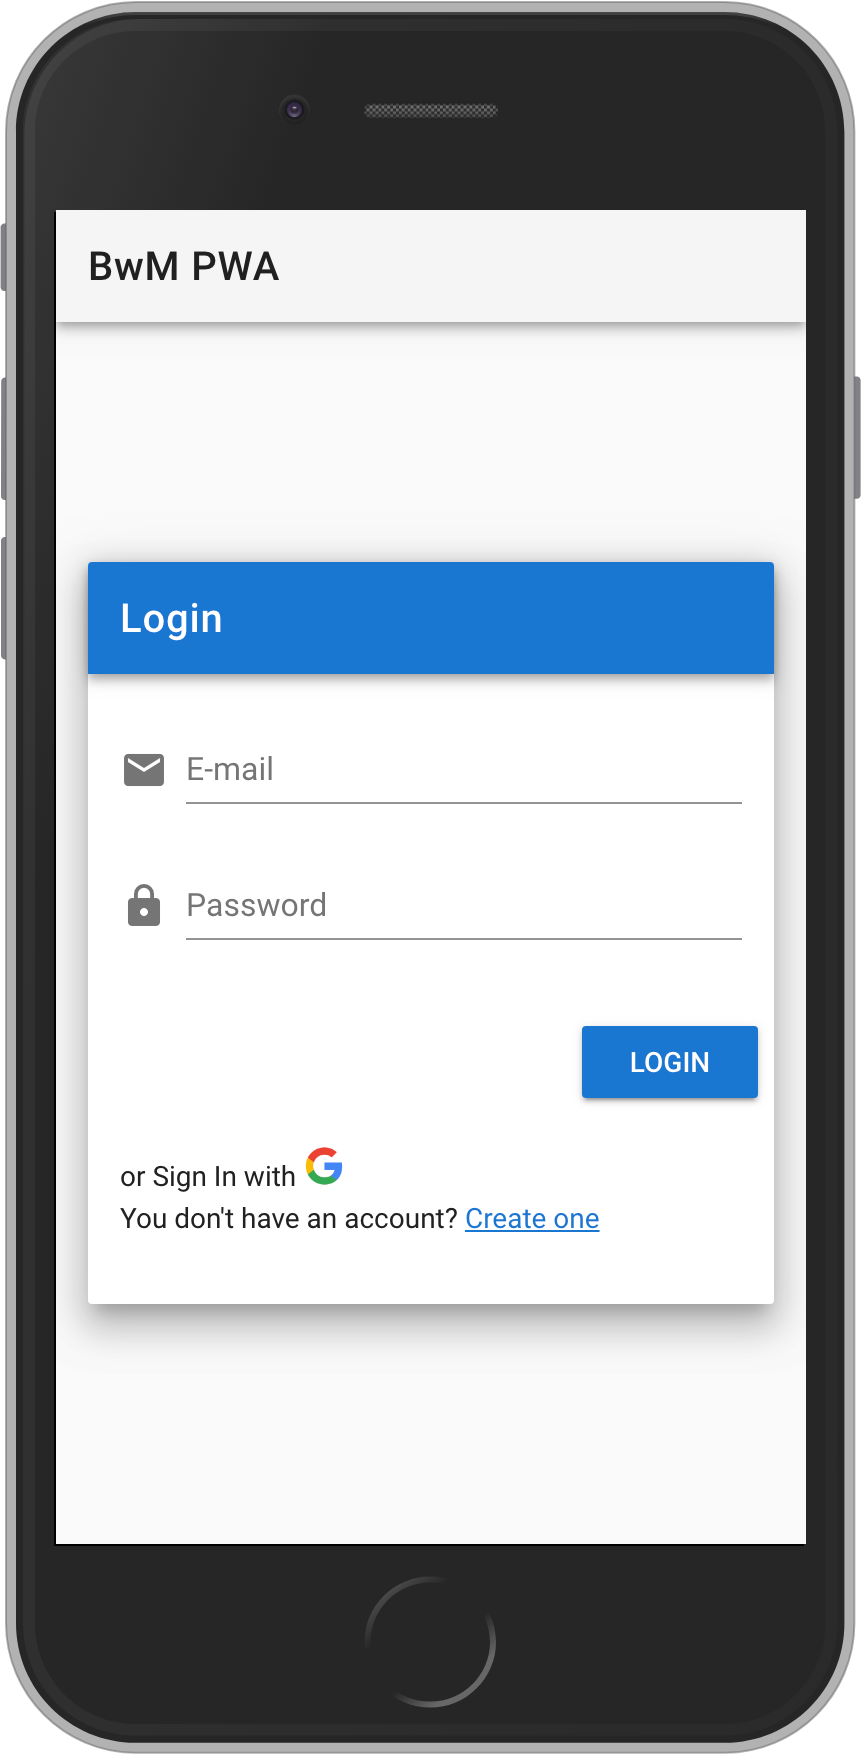
\includegraphics[width=.7\linewidth]{img/screen01}
    \caption{Login screen}
    \label{fig:sub1}
  \end{subfigure}%
  \begin{subfigure}{.5\textwidth}
    \centering
    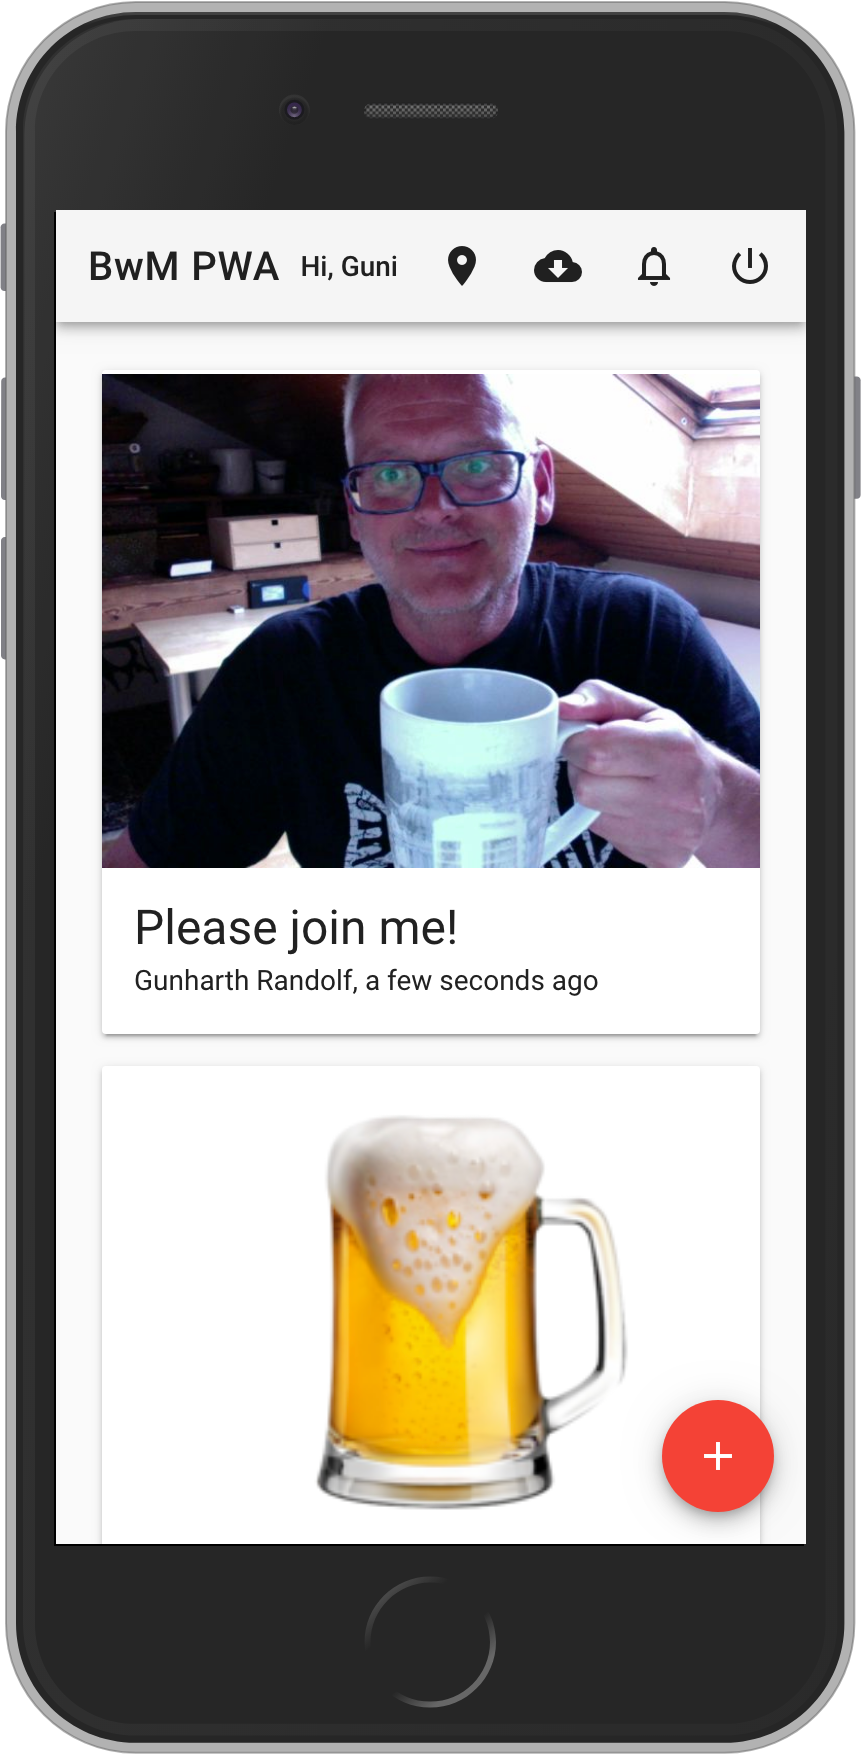
\includegraphics[width=.7\linewidth]{img/screen02}
    \caption{Main app screen}
    \label{fig:sub2}
  \end{subfigure}
  \begin{subfigure}{.5\textwidth}
    \centering
    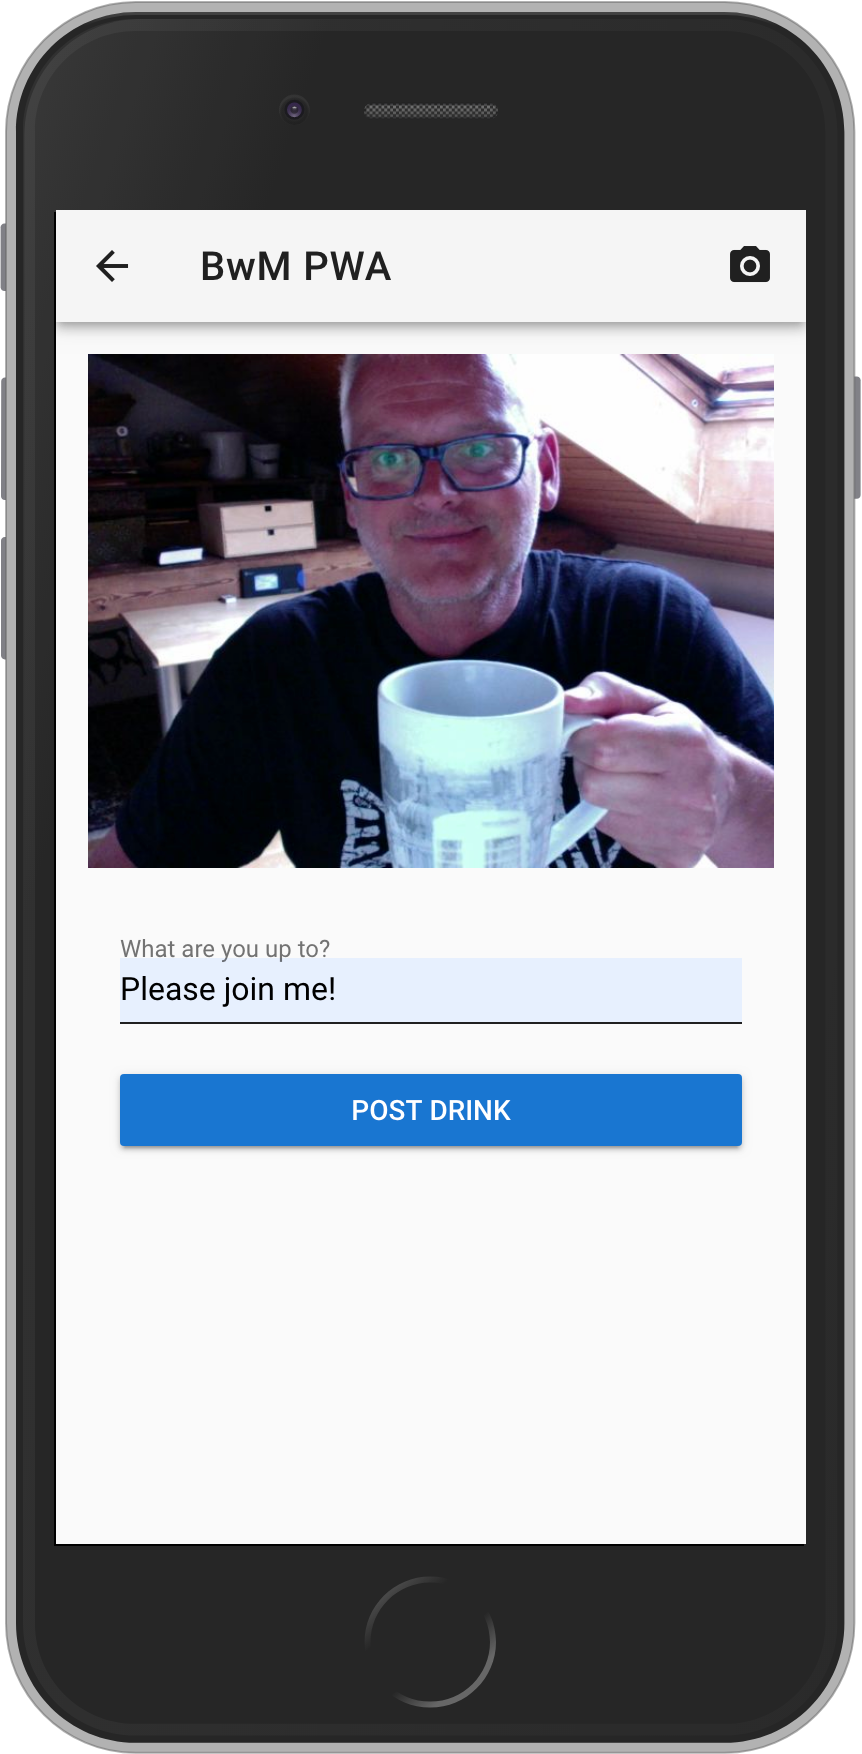
\includegraphics[width=.7\linewidth]{img/screen04}
    \caption{New post screen with photo option}
    \label{fig:sub1}
  \end{subfigure}%
  \begin{subfigure}{.5\textwidth}
    \centering
    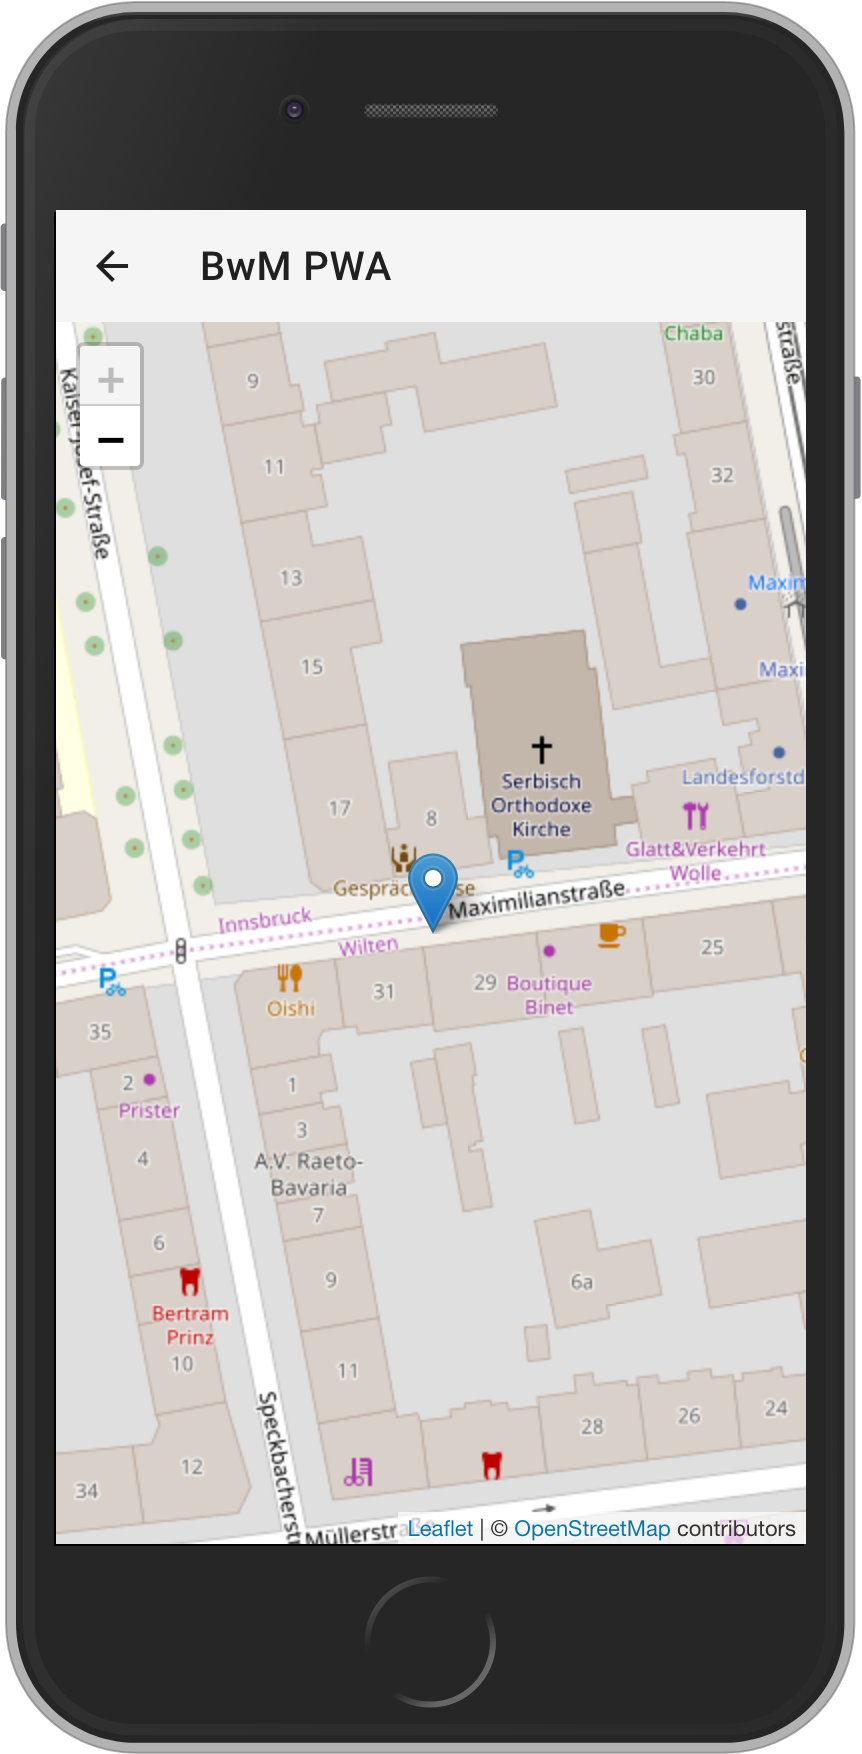
\includegraphics[width=.7\linewidth]{img/screen03}
    \caption{The map}
    \label{fig:sub2}
  \end{subfigure}
  \caption{Frontend screenshots showing main app screens, Vuetify material design components and the map.}
  \label{fig:test}
\end{figure}
\pagebreak

Figure 3 shows the Lighthouse\footnote{\url{https://developers.google.com/web/tools/lighthouse}} Progressive Web App report for the \textit{Beer with Me} PWA.
\fig{img/lighthouse_test}{Lighthouse report}{fig:lighthouse}{1}


\subsection{Cloud Provider and Realtime Functionalities}

For the backend I picked Firebase\footnote{\url{https://firebase.google.com}} as the provider. Around the same time in 2015, when the term Progressive Web Apps was born, Google acquired this San Francisco start-up. Since then Google has expanded upon the original service and integrated it closely into their other cloud ambitions - whereby the Firebase service is dedicated to providing a specialized Platform as a Service (PaaS) for mobile and web applications.

Firebase offers a JavaScript API which is installed through npm. The Firebase CLI enables development directly from the command line. All Firebase services can be configured and maintained through the CLI.

\begin{lstlisting}[language=JavaScript, caption=Firebase configuration and services (firebaseConfig.js), label=lst:firebase-conf]
import firebase from "firebase/app";
import "firebase/firestore";
import "firebase/messaging";
import "firebase/storage";
import "firebase/auth";
import { config } from "@/firebaseCredentials.js";

firebase.initializeApp(config);
let db = firebase.firestore();
db.enablePersistence({ synchronizeTabs: true });
const storage = firebase.storage();
let messaging = null;
if (firebase.messaging.isSupported()) {
  messaging = firebase.messaging();
}
const auth = firebase.auth();
const socialAuth = firebase.auth;
export default {
  db,
  storage,
  messaging,
  auth,
  socialAuth
};
\end{lstlisting}


The following section demonstrates the Firebase services used for the \textit{Beer with Me} PWA.

\textbf{Authentication and Authorization}. Firebase Auth offers multiple methods to authenticate, including email and password and third-party providers like Google. It integrates tightly with other Firebase services and it leverages standards like OAuth 2.0 and OpenID Connect.

\begin{lstlisting}[language=JavaScript, caption=Firebase Auth initiation using VueJS (main.js), label=lst:firebase-auth]
  // Init Firebase auth before Vue inits the App
  firebase.auth.onAuthStateChanged(firebaseUser => {
    if (firebaseUser) {
      store.dispatch("autoSignIn", firebaseUser);
    }
    if (!app) {
      app = new Vue({
        router,
        store,
        render: h => h(App)
      }).$mount("#app");
    }
  });
\end{lstlisting}

\textbf{Realtime Database}. Firebase offers a realtime Database service with Firestore, which stores and syncs data between users and devices using a cloud-hosted, JSON based NoSQL database. An important feature of Firestore in terms of PWAs is offline support and live synchronization.

\begin{lstlisting}[language=JavaScript, caption=Realtime query for new posts (Home.vue), label=lst:firebase-listposts]
firebase.db
  .collection("drinks")
  .orderBy("created_at", "desc")
  .onSnapshot(snapShot => {
    this.drinks = [];
    snapShot.forEach(drink => {
      this.drinks.push({
        id: drink.id,
        url: drink.data().url,
        comment: drink.data().comment,
        author: drink.data().author,
        created_at: drink.data().created_at,
      });
    });
  });
\end{lstlisting}

Photos taken by the user are stored using the Firebase Cloud Storage service, a CDN (Content Delivery Network) driven service by Google tightly integrated with the authentication service. At present there is no offline support available, i.e photos taken offline are not synced to the storage once there is a connection. One solution to this caveat is to save the photo as a base64 encoded string into the Firestore database. Once the actual database query runs, Firebase Functions converts the string to an actual image, stores the file to the Firebase Cloud Storage and saves the resulting image reference back into Firestore.

\begin{lstlisting}[language=JavaScript, caption=Store a photo to Firebase Cloud Storage (Camera.vue), label=lst:firebase-photos]
firebase.storage
  .ref()
  .child(`images/picture-${new Date().getTime()}`)
  .put(blob)
  .then(res => {
    res.ref.getDownloadURL().then(pictureUrl => {
      console.log("File available at", pictureUrl);
    });
  })
\end{lstlisting}

\textbf{Realtime Push Notifications}. The Firebase Cloud Messaging\footnote{\url{https://firebase.google.com/docs/cloud-messaging}} (FCM) service in combination with Firebase Cloud Functions\footnote{\url{https://firebase.google.com/products/functions}} allows to listen for events to send out push notifications to a single user or a group of users.  Functions is a dedicated service that seamlessly ties into the other Firebase offerings.

\begin{lstlisting}[language=JavaScript, caption=Firebase Functions calling the messaging service when a new post is created in the Firestore database(functions/index.js), label=lst:firebase-function]
exports.createDrink = functions.firestore
.document("drinks/{drinkId}")
.onCreate(event => {
  var drink = event.data();
  console.log(drink.comment);
  return axios
    .post(
      "https://fcm.googleapis.com/fcm/send",
      {
        to: "/topics/general",
        priority: "high",
        notification: {
          title: drink.author + " is thirsty!",
          body: drink.comment || "Join in for a drink",
          click_action: "https://bwm.gunicode.com",
          icon: "https://bwm.gunicode.com/img/icons/notification-128x128.png"
        }
      }
});
\end{lstlisting}

Listing the full integration of Firebase Functions into the \textit{Beer with Me} PWA is beyond the scope of this paper. Refer to the codebase at \url{https://github.com/gunharth/bwm} in the functions folder and the relevant sections of the Firebase documentation for messaging\footnote{\url{https://firebase.google.com/docs/cloud-messaging}} and functions\footnote{\url{https://firebase.google.com/docs/function}}

Finally, \textbf{Firebase Hosting} service is used to deploy the demo to \url{https://bwm.gunicode.com}. Using the firebase CLI this is a straight forward process. Once the project is registered as a service through the Firebase CLI new versions of a project can be easily deployed.

\begin{lstlisting}[language=bash, caption=Firebase CLI commands, label=lst:vue-cli]
  # Install the CLI globally through npm
  $ npm install -g firebase-tools
  # login to the firebase service
  $ firebase login
  # register a new project with firebase
  $ firebase init
  # deploy the project to firebase hosting
  $ firebase deploy
\end{lstlisting}
